
\documentclass[twocolumn]{article}
\usepackage{mathpazo}
\usepackage{microtype}
\usepackage{times}

 %%%%%%%%%%%%%%%%%%%%%%%%%%%%%%%%%%%%%%%%%%%%%%%%%%%%%%%%%%%%%%%%%%%%%%%%%%%%%
 %                              My Commands
\newcommand{\bi}{\begin{itemize}}
\newcommand{\ei}{\end{itemize}}
\newcommand{\be}{\begin{enumerate}}
\newcommand{\ee}{\end{enumerate}}
\newcommand{\ii}{\item}
\newtheorem{Def}{Definition}
\newtheorem{Lem}{Lemma}
\usepackage{algorithm}
\usepackage{algorithmicx}
\usepackage{algpseudocode}

\usepackage{graphicx}
\graphicspath{%
        {converted_graphics/}
        {./images/}
}

\usepackage[hangul,nonfrench,finemath]{kotex}
    
\setlength\textwidth{7in} 
\setlength\textheight{9.5in} 
\setlength\oddsidemargin{-0.25in} 
\setlength\topmargin{-0.25in} 
\setlength\headheight{0in} 
\setlength\headsep{0in} 
\setlength\columnsep{18pt}
\sloppy 
 
\begin{document}

\title{
\vspace{-0.5in}\rule{\textwidth}{2pt}
\begin{tabular}{ll}\begin{minipage}{4.75in}\vspace{6px}
\noindent\large {\it KIWI Project}@Data Management Research Section\\
\vspace{-12px}\\
\noindent\LARGE ETRI\qquad  \large Technical Report 14ZS1410-TR-54
\end{minipage}&\begin{minipage}{2in}\vspace{6px}\small
218 Gajeong-ro, Yuseong-gu\\
Daejeon, 305-700, South Korea\\
http:/$\!$/www.etri.re.kr/\\
http:/$\!$/sungsoo.github.com/\quad 
\end{minipage}\end{tabular}
\rule{\textwidth}{2pt}\vspace{0.25in}
\LARGE \bf 빅데이터: 정형 데이터를 위한 분산 저장 시스템 \\
\large Bigtable: A Distributed Storage System for Structured Data
}

\date{}

\author{
{\bf Sung-Soo Kim}\\
\it{sungsoo@etri.re.kr}
}

\maketitle

\begin{abstract}
빅테이블은 수천대 이상의 서버에서 페타(peta) 바이트에 달하는 매우 큰 용량의 데이터를 다루기 위해 디자인된 구조화된 데이터(structured data)를 관리하기 위한 분산 저장 시스템(distributed storage system)이다.
구글의 web indexing, Google Earth, Google Finance와 같은, 많은 구글의 프로젝트들의 데이터가 빅테이블에 저장된다. 
이러한 프로젝트들이 서로 다른 다양한 요구사항들을 빅테이블에 요청하고 있음에도 불구하고, 
빅테이블은 높은 성능과 유연성을 이러한 구글 프로젝트들에 성공적으로 제공하고 있다.
이 논문에서는 빅테이블에서 제공하는 간단한 데이터 모델(simple data model)을 설명하고, 데이터의 레이아웃(layout)과 포맷(format)을 다양하게 제어하는 것, 그리고 빅테이블의 디자인과 구현에 대해 설명하고 있다.
\end{abstract}

\section{Introduction}

%\begin{figure}[!t]
%        \centering
%        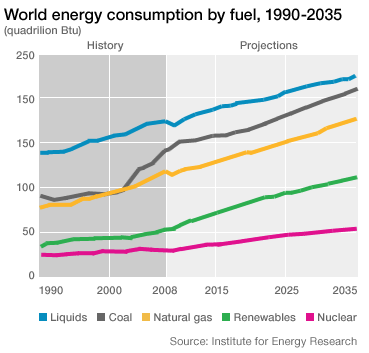
\includegraphics[width=0.33\textwidth]{test}
%        \caption{Caption}
%        \label{fig1}
%\end{figure}
2000년 초부터 구글은 구조화된 데이터(structured data)를 관리하기 위한, 빅테이블이라 불리는 분산 저장 시스템을 디자인하고, 구현하고, 배포했다.
빅테이블은 수천대의 머신(machine)과 페타(peta)바이트의 스케일에서도 신뢰성을 가질 수 있도록 디자인 되었으며, 확장성과 높은 성능, 그리고 유용성등의 목표들을 달성하였다.

빅테이블은 Google Analytics, Google Finance, Orkut, Personalized Search, Writely, Google Earth 등과 같은 60개 이상의 구글 상품(product) 또는 프로젝트에서 이용이 되고 있으며, 이러한 상품들은 간단한 배치 프로세싱에서부터, 최종 유저에게 잠재되어있는 미묘한 데이터를 제공하는 등과 같은 다양한 요구를 수행하기 위해 빅테이블을 사용한다.
 
 여러가지 관점에서 볼때,  빅테이블은 데이터베이스와 닮았다. 왜냐하면, 빅테이블은 데이터베이스의 구현 전략의 많은 부분을 공유하고 있기 때문이다.
 병렬 데이터베이스(\textit{parallel databases})와 메인 메모리 데이터베이스(\textit{main-memory databases})가 확장성과 높은 처리성능(performance)을 달성했지만, 빅테이블은 그러한 시스템과는 다른 인터페이스를 제공한다. 빅테이블은 관계형 데이터 모델(full relational data model)을 지원하지 않는다. 대신에 데이터 레이아웃과 포맷을 다양하게 컨트롤 할 수 있는 간단한 데이터 모델을 제공한다.

데이터는 임의의 문자열 row와 column 이름들로 인덱싱된다. 사용자가 이러한 데이터를 종종 다양한 형태의 구조화된 데이터로 직렬화(serialize)하려고 할지라도, 빅테이블은 이러한 문자열들을 해석되지 않은 문자열들로 취급해 버린다. 사용자는 데이터를 자신들의 주제에 맞는 선택을 통해 컨트롤 할 수 있다. 결국, 빅테이블의 파라미터들은 사용자가 메모리나 디스크로부터 데이터를 제공받는 것을 다이나믹하게 컨트롤 할 수 있도록 해준다.
 
 Section 2 에서는 데이터 모델에 대해 더 자세히 설명하고, Section 3 에서는 사용자 API의 개요를 설명한다. Section 4 에서는 빅테이블에 의존하는 구글의 숨겨진 인프라에 대해 설명한다. Section 5 에서는 빅테이블 구현의 기본적인 것들에 대해 설명하고, Section 6 에서는 빅테이블의 성능을 증명하기 위해 만든 것들에 대해 설명한다. Section 7 에서는 빅테이블의 퍼포먼스의 측정에 대한 내용을 제공하며, 빅테이블이 어떻게 구글에서 활용되고 있는지를 Section 8 에서 설명한다. Section 9 에서는 빅테이블을 디자인하고 지원하기 위해 배웠던 것들에 대해 토론한다. 마지막으로, 빅테이블과 관련된 일들을 Section 10 에서 설명하고, Section 11 에서는 우리의 결론을 발표한다.

\section{Data Model}
빅테이블은 산재해있고(sparse), 분산되어있으며(distributed), 영구적인 다차원의 잘 정리된 맵(multi dimensional sorted map)이다. 이 맵은 row key, column key, timestamp 로 인덱싱 되었다; 맵의 각 value는 해석되지 않은 바이트 어레이(bytes array)이다.

우리는 빅테이블 같은 시스템을 여러가지 용도의 다양한 방법으로 테스트 해보고나서 이 데이터 모델을 우리의 모델로 확정했다. 우리는 다른 많은 프로젝트에서 웹페이지들의 콜렉션과 관련 정보들이 활용될 수 있다는 가정하에 복사본을 유지하기를 원했으며, 이 특별한 테이블을 웹테이블(Webtable)이라고 부르기로 했다. 웹테이블에서 URL들을 row key로 사용할 것이다. column name 들로 웹페이지의 다양한 관점들을 저장하고, contents에 웹페이지의 내용을 저장할 것이다. 그림 1 에서 보이는 것처럼 그 내용이 새로 갱신되었을 때(fetched) column 아래의 timestamps 가 생성될 것이다.
 
Rows
 테이블에서 row key는 최대 64KB의 임의의 문자열이다. (10~100 bytes 가 실제 데이터의 대부분이다.)
하나의 row key는 모든 데이터 읽기와 쓰기의 가장 기본적인 단위이고, 이것은 시스템이 같은 row를 동시에 업데이트 하려는 행동을 보다쉽게 하기위해 디자인 되었다.
 빅테이블은 row key에 의해 사전을 만드는 것으로 데이터를 유지하고, 만들어진 테이블의 row의 범위는 동적으로 분할된다. 이 분할된 각 row의 범위는 테이블릿(tablet)이라고 부르며, 분산과 로드 밸런싱의 기본 단위가 된다. 결론적으로 짧은 row의 범위가 효율적이며, 적은 수의 머신과 통신만으로 데이터를 읽을 수 있다. 사용자는 자신들의 데이터에 접근하기 위해서 row keys를 선택함으로써 이러한 속성(property)를 활용할 수 있다.
예를들면, 웹테이블에서, 같은 도메인을 사용하는 웹페이지들은 URL의 역순으로 구성된 이름에 의해 연속적인 그룹으로 묶여질 수 있다. 예들들면, 우리는 maps.google.com/index.html 을 com.google.maps/index.html 로 저장한다. 같은 도메인에 있는 페이지들을 근처에 있는 머신에 저장하는 것은 도메인을 분석하는 것을 보다 효율적으로 할 수 있도록 해준다.
 
Column Families
 Column keys를 그룹화된 집합으로 묶고 이것을 column families라고 부르며, 이것이 접근 제어(access control)의 가장 기본적인 단위의 형태가 된다. 모든 데이터는 column family 안에 저장되고, 대부분은 같은 형태를 갖는다(우리는 같은 column family를 한꺼번에 압축한다). 데이터가 저장되기 전에 반드시 하나의 column family가 생성되며, 그 family 안에는 column key를 가지게 된다.(홍태바리 주석: 그림1에서 보면 anchor:cnnsi.com 과 anchor:my.look.ca는 anchor 라는 하나의 column family이고 그안의 anchor:cnnsi.com 과 anchor:my.look.ca 가 column key 는 column key 이다.)
하나의 테이블안에 분리된 column family의 수를 적게 만드는 것(수백개 정도 안쪽으로..)이 우리의 의도이고, 동작이 일어나는 동안 families 는 거의 변하지 않는다.(홍태바리 주석: 그림1에서 보면 웹페이지를 저장하기 위해 생성한 column family는 contents, anchor 둘 뿐이다. 물론 실제로는 더 있을 것이다.) 대조적으로, 하나의 테이블안의 column 갯수는 무제한으로 갖게된다.
Column key는 다음과 같은 문법을 갖는다 :
 family:qualifier. Column family의 이름들은 반드시 출력이 가능해야(정해져 있어야) 하지만, qualifier는 임의의 문자열이 될 수 있다. 웹테이블에서 하나의 예들들자면 language를 들 수 있다. 여기서 language는 페이지에 씌여진 언어를 말한다. 우리는 language에서 단 하나의 column key만을 사용했고, 각 웹페이지의 언어 ID만을 저장한다. 또다른 column family 예제로 anchor가 있다. 그림1 에서 보는것처럼 anchor family의 column key들은 각각 하나의 anchor를 나타낸다. 참조하는 사이트의 이름이 qualifier이고, 링크 텍스트가 셀안의 내용이 된다.
 메모리 또는 디스크의 접근제어나 계산의 수행은 column family 레벨에서 실행된다. 웹테이블의 예를들면, 어플리케이션에 따라 제어의 형태가 여러가지로 나타난다 : 기본 데이터에 어떤것을 추가하는 경우, 기본 데이터를 읽는 경우, column family를 생성하는 경우, 존재하는 데이터의 열람만 가능하게 하는 경우(또는 열람 조차도 못하게 하는 경우).
 
Timestamps
 빅테이블의 각 셀은 같은 데이터에 대한 여러개의 버전을 가질 수 있다. 이 버전들은 timestamps 에 의해 인덱싱된다. 빅테이블의 timestamp는 64 비트 정수이다.
 어플리케이션들은 충돌을 피하기 위해서 반드시 유일한 timestamp를 생성해야만 한다. 새롭게 생성된 timestamp가 셀의 위쪽으로 저장되어 가장 먼저 읽혀질 수 있게 된다. 버전별로 정리된 데이터를 관리하는 것을 편하게하기 위해서, 자동적으로 빅테이블의 가비지 콜렉트를 실행할 수 있는 두가지 세팅을 지원한다. 클라이언트는 가장 최근의 n 개의 버전만을 유지하거나, 새로운 데이터만을 유지할 수 있다(예들들면, 최근 7일간의 데이터 값만 유지하는).
웹테이블의 예를들면, 수집된 페이지의 timestamps를 contents 에 저장되도록 세팅해놨다 : 여기서 페이지는 자동적으로 수집되며, 가비지 콜렉션 메카니즘은 페이지마다 최근 세개의 버전을 유지하도록 되어있다.
 
 
\section{API}
 빅테이블 API는 테이블이나 column family를 생성하거나 지울 수 있는 함수들을 제공한다. 또한 클러스터, 테이블, column family, 메타데이타, 접근제어권한과 같은 것들을 변경할 수 있는 함수도 제공한다.
클라이언트 어플리케이션은 빅테이블에 쓰거나 지울 수 있고, 클라이언트 어플리케이션 개인의 row 에서 데이터를 가져오거나, 테이블에 있는 데이터의 하위집합(subset)에 대해서도 이와같은 일을 반복할 수 있다.

%writing_to_bigtable.JPGreading_from_bigtable.JPG
 
 그림 2는 업데이트를 수행하기 위해 RowMutation을 추출하는 C++ 코드를 보여준다. Apply를 호출함으로 웹테이블에 작은 변경이 일어난다 : www.cnn.com 을 anchor에 더하고 다른걸 지운다.
그림 3은 특정 row에 있는 모든 anchor들을 반복적으로 추출하는 Scanner를 사용하는 C++ 코드이다. 클라이언트는 다수의 column family에 사용할 수 있고 rows, columns, timestamps 를 검색할 때 사용하는 몇가지 limit 메카니즘을 가지고 있다. 예들들면, 정규표현식 anchor:*.cnn.com 에 매칭되는 것들만 검색하라는 제한을 두거나, 현재시간으로부터 10일 안의 timestamps 만을 가져오도록 할 수 있다.
빅테이블은 더욱 다양한 방법으로 데이터를 조작하기 위해 몇가지 다른 특성들을 지원하고 있다. 첫째로, 빅테이블은 현재 row key간의 일반적인 트랜잭션을 지원하지 않지만 배치(batch)로 row key를 교차하며 기록할 수 있는 기능을 클라이언트 측에 제공한다. 둘째로, 빅테이블은 cell 이 정수 카운터로 사용되는 것을 허락한다. 결국 빅테이블은 서버의 공간에서 클라이언트가 수행할 수 있는 스크립트를 지원한다. 이 스크립트는 Sawzall이라 불리고, 데이터를 처리하기 위해 구글에서 개발한 언어이다. 현재는, Sawzall 을 기반으로한 API 에서 클라이언트의 스크립트가 빅테이블에 데이터를 쓰는 것을 허락하지 않는다. 그러나, 애매한 표현들에 대한 필터링과 다양한 연산자들에 대한 요약을 클라이언트에 제공하고 있다.
 빅테이블은 구글에서 대용량 병렬 처리를 하기위해 개발한 프레임웍인 MapReduce룰 사용할 수 있다. 우리는 빅테이블에서 input source 와 output target 의 경우 모두에 MapReduce job을 사용하기 위해 wrapper를 사용했다.
 
\section{Building Blocks}
빅테이블은 구글의 여러개의 다른 인프라의 조각들로 구성되어 있다. 빅테이블은 로그와 데이터 파일들을 저장하기 위해 분산 구글파일 시스템을 사용한다. 빅테이블은 일반적으로 다양한 분산 어플리케이션들이 실행되는 머신들의 공유된 풀(pool)에서 동작하고, 때로는 다른 어플리케이션들의 프로세스에서 사용하는 머신을 공유하기도 한다. 빅테이블은 job을 스케쥴링하고, 자원을 관리하고, 머신을 공유하고, 머신 오류를 다루고, 머신의 상태를 모니터링하는 부분들을 클러스터 운영 시스템에 의존한다.
 내부적으로 빅테이블의 데이터를 저장하기 위해 구글 SSTable 이라는 파일 포맷을 사용한다. 하나의 SSTable은 key 값들부터 그에 해당하는 value 값들까지 영구적으로 변하지않는 정렬된 맵(ordered immutable map)을 제공하고, 여기에 사용되는 key 값들과 value 값들은 임의의 바이트 문자열이 된다. 구체화된 key 값으로, 관련된 value값을 가져오거나 특정영역의 key/value 쌍을 반복적으로 가져올 수 있는 연산자(operation)들이 제공된다. 내부적으로, 각 SSTable 들은 연속된 블록(blocks)들을 가지고 있다(일반적으로 각 블록은 64KB 이지만 이것은 조절이 가능하다). SStable의 마지막에 저장된 블록 인덱스는 블록의 위치를 찾아내기 위해서 사용된다 : SSTable이 오픈될때 인덱스가 메모리에 올라간다.
단일 디스크 검색으로도 룩업(lookup)이 실행될 수 있다 : 먼저 메모리에 있는 인덱스에서 바이너리 검색을 통하여 적절한 블록을 찾은 다음, 그리고나서 디스크로 부터 적절한 블록을 읽는 것이다. 추가적으로 SSTable을 메모리에 완전히 매핑하고, 디스크 검색을 전혀하지 않는 방법 또한 가능하다.
빅테이블은 Chubby라고 불리는 지속적인 분산 락(lock) 서비스에 의존한다. Chubby 서비스는 다섯개의 활동적인 리플리카(replica)로 구성되어있고, 여기서 하나가 선출되어 마스터가 되고, 들어오는 요청에 능동적으로 반응하게 된다. 리플리카의 과반수 이상이 살아있고, 다른 것들과 통신이 가능할 때 그 서비스는 살아있다고 할 수 있다. Chubby는 리플리카를 지속적으로 유지하고 실패에 대응하기 위해 Paxos 알고리즘을 사용한다. Chubby는 디렉토리들과 작은 파일들로 구성된 네임스페이스를 제공한다. 각각의 디렉토리 또는 파일들은 하나의 락(Lock)으로 사용될 수 있고, 파일에 읽고 쓰는 작업들은 기본적인 작업이 될 수 있다. Chubby 클라이언트 라이브러리는 Chubby 파일의 캐싱(cashing)을 지속적으로 제공한다. 각각의 Chubby 클라이언트들은 하나의 Chubby 서비스에 하나의 session을 갖게되고, session은 session 만료 시간내에 유효 시간을 연장하지 못하면 소멸하게 된다. 클라이언트의 session이 만료되면 모든 락과 열린 핸들을 모두 잃게된다. Chubby 클라이언트는 변경 또는 session의 만료를 알리기 위해서 Chubby 파일과 디렉토리의 콜백(callback)을 등록할 수 있다.
빅테이블은 다양한 용도로 Chubby를 사용한다 : 하나의 활성화된 마스터가 있는지를 보장하는 것과, 빅테이블 데이터의 bootstrap 위치를 저장하는 것, 새로운 타블렛(tablet) 서버를 발견하는 것과 죽은 서버에대한 최종 승인을 하는 것, 빅테이블의 스키마 정보를 저장하는 것, 그리고 접근제어 리스트를 저장하는 것. 만약에 일정기간 동안 Chubby가 이용가능하지 않게된다면, 빅테이블도 이용불가능한 상태가 된다.
 
\section{Implementation}
빅테이블은 세가지 중요한 구성요소로 구현이 된다 : 모든 클라이언트로 연결된 하나의 라이브러리, 하나의 마스터 서버, 그리고 많은 타블렛 서버들.
타블렛 서버들은 부하(workloads)에 따른 적절한 조절을 위해서 클러스터에의해 동적으로 추가되거나 제거가 될 수 있다. 마스터는 타블렛을 타블렛 서버에 할당하거나, 추가되거나 만료된 타블렛 서버를 검출하고, 타블렛 서버의 로드 밸런싱과 구글파일시스템에서의 가비지 콜렉션을 담당하게된다. 게다가, 테이블과 컬럼 패밀리의 생성과 같은 스키마의 변경 또한 핸들링한다. 일반적으로 각각의 타블렛 서버는 서버당 수십에서 수천개의 타블렛을 관리한다. 타블렛 서버는 가지고 있는 타블렛들의 읽기와 쓰기에 대한 요청과, 타블렛의 크기가 너무 커진 경우에 대한 관리를 한다.
대부분의 단일 마스터 분산 저장 시스템에서, 클라이언트 데이터는 마스터를 거쳐서 이동하지 않는다 : 클라이언트는 읽기와 쓰기를 수행하기위해 타블렛 서버와 직접 통신한다. 따라서, 빅테이블 클라이언트는 타블렛 위치 정보를 위해 마스터에 의존하지 않고, 대부분의 클라이언트들은 마스터와 절대 통신하지 않는다. 결론적으로 봤을때, 마스터는 거의 로드가 걸리지 않는다.
빅테이블의 클러스터는 많은 테이블들을 저장한다. 각 테이블은 타블렛의 집합으로 구성되고, 각각의 타블렛은 row range들로 조합된 모든 데이터를 가지고 있다. 테이블의 크기가 커지면, 자동적으로 여러개의 타블렛으로 나눠지고, 대략 그 크기는 100~200MB 정도가 된다.
 
\subsection{Tablet Location}
우리는 타블렛 위치 정보를 저장하기 위해서 B+- 트리의 그것과 비슷한 3 단계의 계층구조를 사용한다.

% tablet_location_hierachy.JPG

 첫번째 단계는 Chubby에 저장된 루트 타블렛(root tablet)의 위치를 가지고 있는 파일이다. 루트 타블렛은 특별한 METADATA 테이블에 모든 타블렛들의 위치를 가지고 있다. 각각의 METADATA 타블렛은 유저 타블렛들의 집합에 대한 위치를 가지고 있다. 루트 타블렛은 단지 METADATA 테이블의 첫번째 타블렛에 불과하지만, 타블렛 위치 계층구조가 3단계 이상을 가지지 않게하기 위해 특별하게 취급된다. - 루트 타블렛은 절대 쪼개지지 않는다.
METADATA 테이블은 타블렛의 테이블 식별자와 마지막 row를 인코딩한 row key 아래에 타블렛 위치를 저장한다. 각각의 METADATA row 는 메모리에 있는 데이터의 대략 1KB를 저장한다. 그다지 크지 않은 128MB METADATA 타블렛 사이즈로, 우리의 3단계 계층구조의 위치 스키마는 2의 34제곱 타블렛들의 어드레스를 하는 것이 가능하다(또는 128MB 타블렛에서 2의 61 제곱 바이트).
클라이언트 라이브러리는 타블렛 위치를 캐쉬한다. 만약 클라이언트가 타블렛의 위치를 모르거나, 캐쉬된 위치정보가 잘못되었다는 것을 발견하면 타블렛 계층구조를 타고 위로 올라가게 된다. 만약 클라이언트의 캐쉬가 비어있으면, 위치 알고리즘은 Chubby로 부터 읽어오는 것을 포함하여 네트워크를 3번 왕복하는 것을 요구한다. 만약 캐쉬의 정보가 오래되었다면, 위치 알고리즘은 네트워크를 여섯번 왕복하도록 만든다. 왜냐하면, METADATA 타블렛들이 빈번하게 움직이지 않는다는 가정하에, 빠뜨렸던 것을 발견할 수 있기 때문이다.  타블렛 위치가 메모리에 저장되기 때문에 구글파일시스템(GFS)에 접근할 필요가 없긴 하지만, 앞으로는 클라이언트 라이브러리가 타블렛 위치들을 미리 패치하도록 함으로써 이러한 비용을 점점 줄여나갈 것이다 : 메타데이타 테이블을 읽을때는 반드시 하나 이상 타블렛의 메타데이터를 읽는다.
우리는 메타데이터 테이블의 각 타블렛에서 발생하는 모든 이벤트 로그와 같은 2차 정보들을 저장한다. 이러한 정보는 디버깅이나 성능을 분석하는데 매우 유용하다.
 
\subsection{Tablet Assignment}
타블렛들은 각각 하나의 타블렛 서버에 할당된다. 마스터는 살아있는 타블렛 서버들을 확인하고, 타블렛 서버에 할당되어진 타블렛들이 현재 수행하는 작업을 추적하고, 작업이 할당되지 않은 타블렛 또한 확인한다.


\end{document}
